\documentclass[11pt]{article}

\usepackage[T1]{fontenc}
\usepackage{lmodern}
\usepackage[margin=1in]{geometry}
\usepackage{amsmath,amssymb,amsthm}
\usepackage{graphicx}
\usepackage{booktabs}
\usepackage{xcolor}
\usepackage[authoryear,round]{natbib}
\usepackage[colorlinks=true,allcolors=blue!60!black]{hyperref}

\graphicspath{{../paper/figures/}}

\newtheorem{proposition}{Proposition}
\theoremstyle{remark}
\newtheorem*{remark}{Remark}

\title{When Does Entry Offset Displacement?\\A Note on AI, Firm Scale and Entrant Quality\thanks{Code, data and the scripts behind every figure and number are at \url{https://github.com/gspivey/ai-employment-offset}. The views expressed are the author's own and do not represent those of any employer. Large-language-model tools were used to assist with coding and editing; the economic content and its interpretation are the author's own.}}
\author{Gerard Spivey\\\href{mailto:gs@gspivey.com}{gs@gspivey.com}}
\date{Draft --- November 2026}

\begin{document}
\maketitle

\begin{abstract}
\noindent
AI can lower the labor demand of the firms that adopt it while lowering the cost of starting new firms. I derive, at a fixed wage, the condition under which entry offsets displacement at adopters. The condition depends on four objects: the adopters' share of employment, the gap between the labor-AI elasticity of substitution and the firm's scale elasticity, the response of entry to entry costs, and the productivity of entrants. I then show that a shift in entrant productivity raises entrant labor demand by more than an equal proportional cut in entry costs whenever the scale elasticity exceeds the elasticity of the pool of potential founders, and I state when the ranking reverses.
\end{abstract}

\medskip
\noindent\textbf{JEL:} D22, J23, L26, O33. \quad \textbf{Keywords:} artificial intelligence, entry, labor demand, elasticity of substitution.

\section{Introduction}

Most work on AI and jobs holds the set of firms fixed. Two recent papers instead study the entry margin directly. \citet{bena2026prompted} find that industries more exposed to generative AI saw about 20\% more startup formation, with smaller entrants but net job and wage growth among new firms. \citet{gupta2026generative} find that exposed startups cut junior jobs while new firm formation kept aggregate startup employment unchanged. Neither studies displacement at large incumbents, which is where automation concentrates when adoption carries a fixed cost \citep{hubmer2021typical}.

This note gives a compact analytical frame for that missing link. It makes three points. First, the firm-level condition for AI to raise an adopter's headcount is the textbook scale-versus-substitution condition of derived demand \citep{hamermesh1993labor}; I state it for a general scale elasticity and normalize the technology so that the substitution elasticity does not also set the size of the shock. Second, I derive the industry-level condition under which entry offsets displacement. Third, I show why entrant quality matters more than entry costs, and when it does not.

All results are statements about labor demand at a fixed wage. They are not equilibrium employment effects, and they abstract from business stealing among incumbents, which firm-level evidence on automation shows can be large \citep{acemoglu2020competing,koch2021robots}. A companion quantitative paper, in progress, is being built to add those margins.

\section{Setup}

An industry has heterogeneous firms indexed by productivity $z$ and faces a fixed wage $w$. A firm's demand for its composite input $X$ satisfies $X = A_0 (z/c)^{\theta}$, where $c$ is the unit cost of $X$ and $\theta > 1$ is the \emph{scale elasticity}: the elasticity of the firm's input demand with respect to its unit cost. Under span of control, $y = zX^{\alpha}$, $\theta = 1/(1-\alpha)$ \citep{lucas1978size}; under monopolistic competition with demand elasticity $\varepsilon$, $\theta = \varepsilon$.

The composite combines labor $n$ and AI services $a$ with elasticity of substitution $\sigma > 1$, normalized so that a firm without AI has unit cost $w$:
\begin{equation}\label{eq:cost}
  c = \bigl(w^{1-\sigma} + r^{1-\sigma}\bigr)^{1/(1-\sigma)},
\end{equation}
where $r$ is the effective price of AI services. Cost minimization gives $n = (c/w)^{\sigma} X$. Write $k \equiv c/w < 1$ for an adopter's unit-cost ratio.

\paragraph{Normalization.} In \eqref{eq:cost}, holding $r$ fixed while varying $\sigma$ changes $k$ as well: an input priced like labor halves unit cost at $\sigma = 2$ but cuts it by only 16\% at $\sigma = 5$. Comparative statics in $\sigma$ at a fixed $r$ therefore mix substitutability with the size of the shock, a known problem with CES comparisons \citep{klump2000growth,leonledesma2010identifying}. Throughout I hold $k$ fixed when varying $\sigma$, which amounts to letting $r$ adjust with $\sigma$.

\paragraph{Entry.} Potential entrants arrive with mass $M = M_0 c_e^{-\eta}$, where $c_e$ is the sunk entry cost and $\eta \ge 0$ the elasticity of the founder pool. Each draws $\ln z \sim N(\mu, s^2)$ and enters if its value $V(z) = B z^{\theta} - F$ covers $c_e$, where $F$ is the present value of fixed costs \citep{hopenhayn1992entry}. Entrants that do not adopt AI demand labor $n = D z^{\theta}$. Labor demand of an entry cohort is then
\begin{equation}\label{eq:NE}
  N_E = M D \, e^{\theta\mu + \theta^2 s^2/2}\, \bar\Phi(v), \qquad v = \frac{\ln z_e - \mu}{s} - \theta s,
\end{equation}
where $\ln z_e = \theta^{-1}\ln[(c_e + F)/B]$ is the entry cutoff, $\bar\Phi = 1-\Phi$, and \eqref{eq:NE} uses the truncated moment of the lognormal.

\section{The firm-level condition}

\begin{proposition}[Adopter headcount]\label{prop:firm}
At a fixed wage and productivity, adoption multiplies a firm's labor demand by $k^{\sigma - \theta}$. Adoption raises headcount if and only if $\sigma < \theta$.
\end{proposition}

\noindent This is an application of the Hicks--Marshall rule: a cheaper input raises demand for its substitute when the scale response, here $\theta$, outweighs substitution. It is not new, but two features matter below. The threshold is a statement about $\theta$, not about AI alone: at $\alpha = 0.64$ it is 2.78, while returns to scale near 0.85, common in calibrations with capital \citep{atkeson2005modeling,restuccia2008policy}, put it at 6.67. And with $k$ held fixed, $\sigma$ moves only the exponent.

\section{The industry condition with entry}

Let baseline industry labor demand be $N = N_A + N_O + N_E$, where $N_A$ is demand at incumbents that adopt, $N_O$ at incumbents that do not, and $N_E$ at the entry cohorts over the horizon of interest. Write $a = N_A/N$ and $e = N_E/N$. The AI shock (i) lowers adopters' unit-cost ratio to $k$, (ii) scales the entry cost by $\kappa \le 1$, (iii) shifts entrants' mean log productivity by $\Delta \ge 0$, and (iv) changes entrants' labor per unit of input by a factor $\ell$ ($\ell = 1$ if entrants do not adopt; $\ell = k_E^{\sigma-\theta}$ if they adopt at cost ratio $k_E$). Non-adopting incumbents are unaffected at the fixed wage.

\begin{proposition}[Industry offset condition]\label{prop:industry}
Industry labor demand changes by
\begin{equation}\label{eq:dN}
  \frac{\Delta N}{N} = a\bigl(k^{\sigma-\theta} - 1\bigr) + e\,(G_E - 1),
  \qquad
  G_E = \kappa^{-\eta}\, e^{\theta\Delta}\, \frac{\bar\Phi(v')}{\bar\Phi(v)}\,\ell,
\end{equation}
with $v' = v - \Delta/s + \theta^{-1} s^{-1}\ln\bigl(1 - \omega_c(1-\kappa)\bigr)$ and $\omega_c = c_e/(c_e+F)$. Hence:
\begin{enumerate}
  \item[(i)] If $\sigma \le \theta$, adopters do not shed labor, and labor demand rises whenever $G_E \ge 1$.
  \item[(ii)] If $\sigma > \theta$, entry offsets displacement if and only if $G_E \ge 1 + (a/e)\bigl(1 - k^{\sigma-\theta}\bigr)$.
  \item[(iii)] The smallest entrant-productivity shift that delivers offset, $\Delta^*$, rises with $\sigma$ above $\theta$, with $a/e$ and with the adopters' cost saving $1-k$, and falls with $\eta$ and with the entry-cost cut. As $\sigma \to \infty$ it converges to a level no greater than $\theta^{-1}\bigl[\ln(1 + a/e) + \eta\ln\kappa - \ln\ell\bigr]$.
\end{enumerate}
\end{proposition}

\begin{proof}[Proof sketch]
Equation \eqref{eq:dN} follows from Proposition~\ref{prop:firm} and from \eqref{eq:NE}: $M$ scales by $\kappa^{-\eta}$, $\mu$ rises by $\Delta$, and the cutoff moves by $\theta^{-1}\ln[(\kappa c_e + F)/(c_e+F)]$. For (ii), set $\Delta N \ge 0$. For (iii), $G_E$ is increasing in $\Delta$ (both $e^{\theta\Delta}$ and $\bar\Phi(v')$ rise), and the right side of (ii) is increasing in $\sigma$ because $k < 1$, so the root $\Delta^*$ rises with $\sigma$. The selection ratio is at least one for $\Delta \ge 0$ and $\kappa \le 1$, so dropping it gives the stated upper bound on the limit, where $k^{\sigma-\theta} \to 0$.
\end{proof}

\noindent The condition makes the offset question concrete. Displacement is weighted by how much employment sits at adopters relative to entrants, $a/e$, which is large when adoption is concentrated in big incumbents. Cheaper entry enters only through $\eta\ln(1/\kappa)$, while entrant productivity is amplified by $\theta$. Figure~\ref{fig:boundary} plots $\Delta^*(\sigma)$ for three values of $a/e$ and three values of $\theta$: raising $\theta$ moves the threshold right \emph{and} flattens the curve, because the same scale elasticity that protects adopters' headcount also magnifies entrant productivity.

\begin{figure}[t]
  \centering
  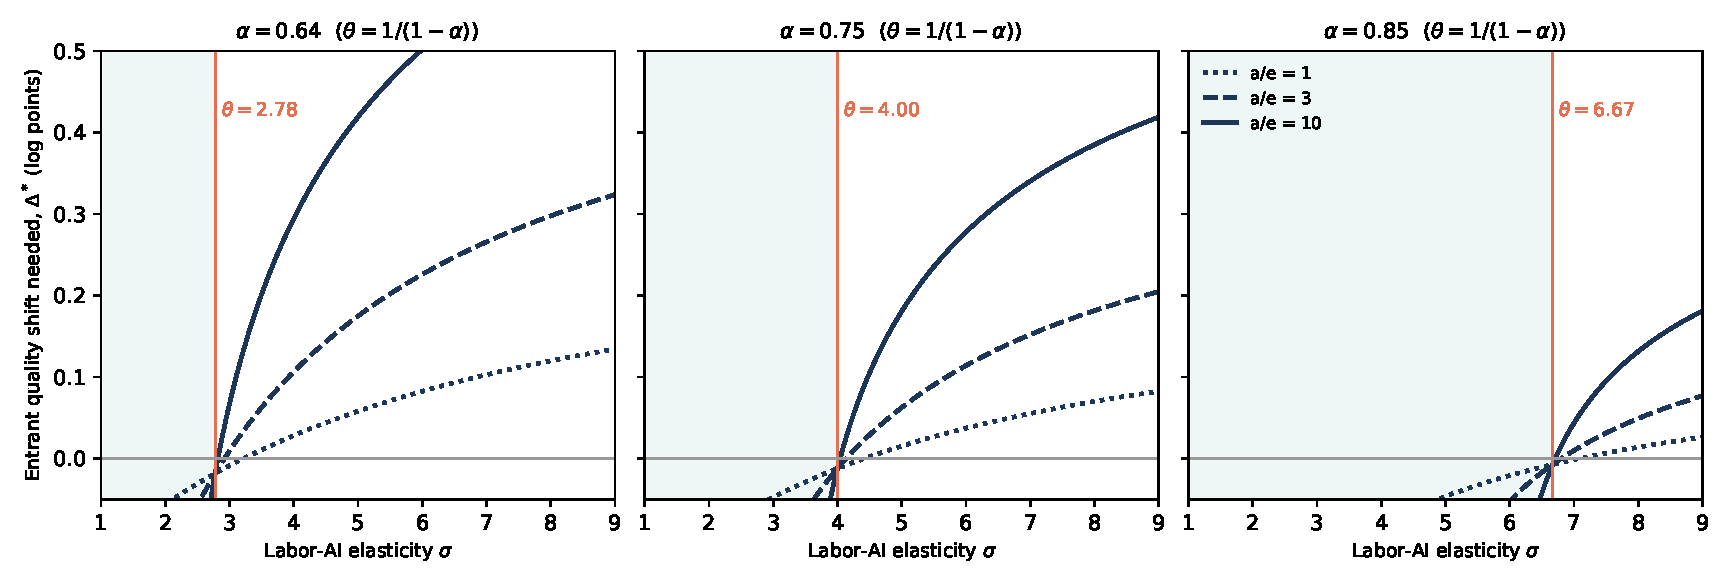
\includegraphics[width=\linewidth]{note_boundary}
  \caption{Entrant productivity shift $\Delta^*$ needed for entry to offset displacement (Proposition~\ref{prop:industry}), by $\sigma$, for $a/e \in \{1, 3, 10\}$ and $\theta = 1/(1-\alpha)$ at three values of $\alpha$. Shaded: $\sigma \le \theta$, where adopters do not shed labor. Illustrative values: $k = 0.8835$ (an 11.65\% cost saving), $\kappa = 0.85$, $\eta = 0.3$, $s = 0.6$, 70\% of potential entrants entering before the shock, $\omega_c = 1$, $\ell = 1$. Source: \texttt{scripts/note\_regime\_boundary.py}.}
  \label{fig:boundary}
\end{figure}

\section{Entrant quality versus entry costs}

\begin{proposition}[Quality versus cost]\label{prop:quality}
The elasticities of entry-cohort labor demand \eqref{eq:NE} with respect to entrant quality and to the entry cost are
\begin{equation}\label{eq:elast}
  E_q \equiv \frac{\partial \ln N_E}{\partial \mu} = \theta + \frac{\lambda(v)}{s},
  \qquad
  E_c \equiv -\frac{\partial \ln N_E}{\partial \ln c_e} = \eta + \frac{\omega_c\,\lambda(v)}{\theta s},
\end{equation}
where $\lambda(v) = \phi(v)/\bar\Phi(v)$. Per log point, entrant quality raises entry-cohort labor demand by more than an entry-cost cut whenever $\theta \ge \eta$. The ranking reverses only if $\eta > \theta + (\lambda(v)/s)(1 - \omega_c/\theta)$.
\end{proposition}

\begin{proof}[Proof sketch]
Differentiate \eqref{eq:NE}. A higher $\mu$ raises the truncated moment one-for-one with $\theta$ and lowers the standardized cutoff by $1/s$; a higher $c_e$ lowers $M$ with elasticity $\eta$ and raises $\ln z_e$ by $\omega_c/\theta$. Then $E_q - E_c = (\theta - \eta) + (\lambda/s)(1 - \omega_c/\theta)$, and $\omega_c \le 1 < \theta$.
\end{proof}

\noindent The ranking rests on two numbers that are rarely measured, $\theta$ and $\eta$, and I want to be explicit about that. At the illustrative values in Figure~\ref{fig:boundary} and $\theta = 2.78$, $\lambda(v) = 0.037$, so $E_q = 2.84$ and $E_c = 0.32$. A 0.10 log-point gain in entrant productivity raises entry-cohort labor demand by 32.7\%; a 20\% cut in entry costs raises it by 7.4\%. Almost all of the gap comes from $\theta/\eta$; the selection terms are small because most potential entrants already clear the cutoff. A very elastic founder pool, or a scale elasticity near one, would narrow or reverse the ranking.

\section{Illustration}

Figure~\ref{fig:sim} shows the same logic in a simulated firm-dynamics economy (about 175,000 workers, endogenous entry and exit, size-selective adoption), with $k$ held fixed across $\sigma$ and ten seeds per cell. The model is not calibrated, so the numbers are illustrative. Labor demand falls to the right and rises with entrant quality, and the boundary between the two regions moves up with $\sigma$, as Proposition~\ref{prop:industry} predicts. Without the normalization the same simulation shows a spurious plateau at high $\sigma$, because a lower $\sigma$ there also means a much larger cost shock.

\begin{figure}[t]
  \centering
  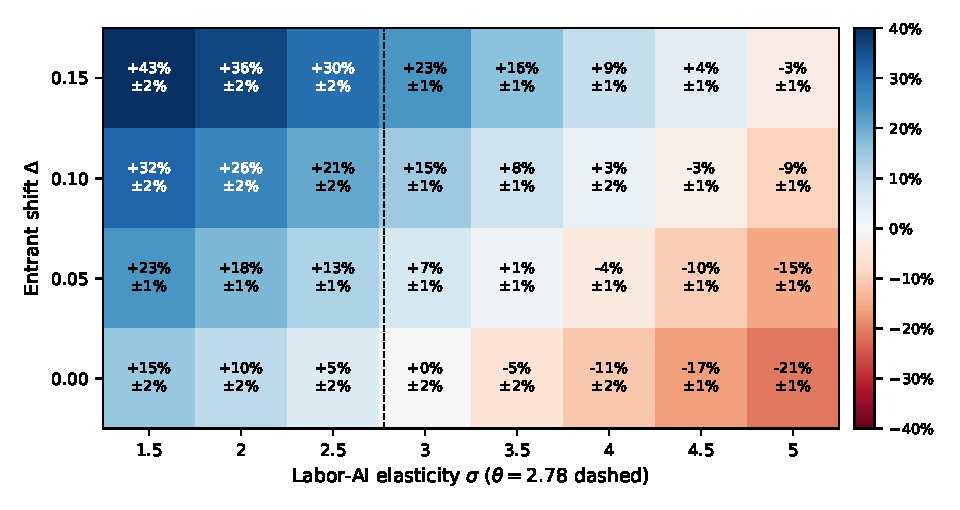
\includegraphics[width=0.85\linewidth]{note_regime_sim}
  \caption{Simulated net change in labor demand relative to an identical economy without AI, by $\sigma$ and entrant productivity shift $\Delta$; mean over ten seeds, with standard errors. Adopters' reference cost saving is fixed at 11.65\% for every $\sigma$; $\alpha = 0.64$; 15\% entry-cost cut; wage fixed. Source: \texttt{scripts/regime\_map.py}, \texttt{scripts/plot\_note\_regime.py}.}
  \label{fig:sim}
\end{figure}

\section{Testable implications}

\begin{enumerate}
  \item \textbf{The sign of $\sigma - \theta$ at adopters.} Within-firm employment responses to falling AI costs identify the sign. Early survey evidence finds few AI-driven employment changes, but more declines among firms that deploy AI more deeply \citep{bonney2026}.
  \item \textbf{Entrant quality.} Proposition~\ref{prop:quality} says offset depends on whether AI-native entrants are more productive than the entrants they replace, not on whether there are more of them. Matched comparisons of AI-native and other startups \citep{kim2026ainative,gupta2026generative} can test this directly.
  \item \textbf{Employer formation, not applications.} The relevant entry response is in employer formations and entrant employment. Business applications can rise for reasons that carry no labor demand, including displaced workers registering as contractors.
\end{enumerate}

\section{Conclusion}

Whether entry offsets displacement is governed by a short list of measurable objects: the gap between substitution and scale, the employment share of adopters relative to entrants, and the productivity of entrants. Cheaper entry matters much less than its prominence in policy debates suggests, unless the founder pool is unusually elastic. A calibrated equilibrium model, in which wages, prices and business stealing respond, is needed to turn these conditions into magnitudes; the companion paper is being developed to take that step.

\bibliographystyle{plainnat}
\bibliography{references}

\end{document}
